\documentclass[11pt]{article}

% ---------- Packages ----------
\usepackage[margin=1in]{geometry}
\usepackage{amsmath,amsthm,amssymb}
\usepackage{mathtools}
\usepackage{physics}
\usepackage{siunitx}
\usepackage{graphicx}
\usepackage{float}
\usepackage{booktabs}
\usepackage{enumitem}
\usepackage{fancyhdr}
\usepackage{titlesec}
\usepackage{hyperref}
\usepackage{tcolorbox}
\usepackage{listings}
\usepackage{xcolor}
\usepackage{bbm}
\usepackage{sgame}

% Define colors
\definecolor{codegreen}{rgb}{0,0.6,0}
\definecolor{codepurple}{rgb}{0.58,0,0.82}
\definecolor{backcolour}{rgb}{0.95,0.95,0.92}

% ---------- Hyperref Setup ----------
\hypersetup{
    colorlinks=true,
    linkcolor=blue,
    urlcolor=blue,
    citecolor=blue
}

% ---------- Header/Footer ----------
\pagestyle{fancy}
\fancyhf{}
\lhead{\textbf{\course}}
\rhead{\textbf{\assignment}}
\cfoot{\thepage}

% ---------- Custom Commands ----------
\newcommand{\course}{ASEN 5264 - DMU}
\newcommand{\assignment}{Homework \#6}
\newcommand{\studentname}{Bijan Jourabchi}

\newcommand{\R}{\mathbb{R}}
\newcommand{\E}{\mathbb{E}}
\newcommand{\Var}{\mathrm{Var}}
\newcommand{\Cov}{\mathrm{Cov}}

% Boxed answer environment
\newtcolorbox{answerbox}{
    colback=gray!5,
    colframe=gray!50,
    title=Answer,
    fonttitle=\bfseries
}

% Problem section format
\titleformat{\section}{\large\bfseries}{Problem \thesection:}{0.5em}{}

% ---------- Code Style ----------
\lstset{
    basicstyle=\ttfamily\small,
    keywordstyle=\color{blue},
    commentstyle=\color{green!50!black},
    stringstyle=\color{orange},
    breaklines=true,
    frame=single
    extendedchars=true,
    literate={π}{{$\pi$}}1 {γ}{{$\gamma$}}1
}

% ---------- Document ----------
\begin{document}

% ---------- Title Block ----------
\begin{center}
    {\LARGE \textbf{\course}} \\[6pt]
    {\Large \assignment} \\[10pt]
    \studentname \\
\end{center}

\vspace{1em}
\hrule
\vspace{1em}

% Define Julia language manually
\lstdefinelanguage{Julia}{
  keywords={abstract, break, case, catch, const, continue, do, else, elseif,
      end, export, false, for, function, global, if, import, in, let, local,
      macro, module, otherwise, quote, return, struct, switch, true, try,
      type, typealias, using, while, mutable},
  keywordstyle=\color{blue}\bfseries,
  comment=[l]{\#},
  morecomment=[n]{\#=}{=\#},
  commentstyle=\color{codegreen}\ttfamily,
  stringstyle=\color{codepurple}\ttfamily,
  morestring=[b]',
  morestring=[b]"
}

% General Listing Settings
\lstset{
    language=Julia,
    backgroundcolor=\color{backcolour},   
    basicstyle=\ttfamily\small,
    breaklines=true,                 
    numbers=left,                    
    numbersep=5pt,                  
    frame=single
}

% =====================================================
\section{}

\begin{enumerate}[label = \alph*)]
    \item 

        
    \item
        \begin{figure}[H]
            \centering
            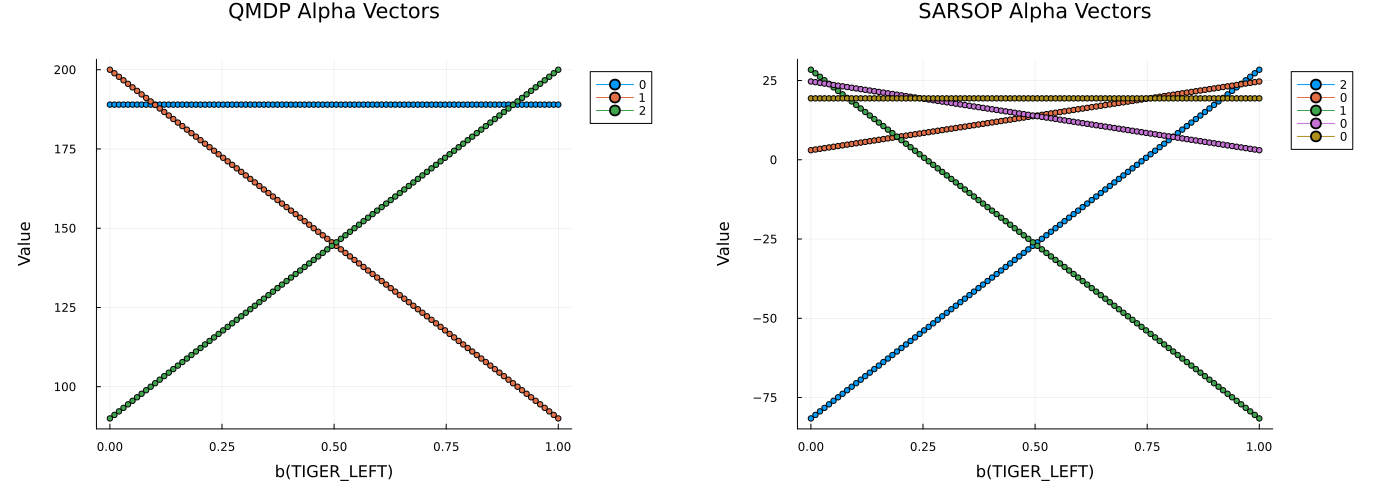
\includegraphics[width=\textwidth, height=0.25\textheight, keepaspectratio]{alpha_vectors_comparison.png}
            \caption{QMDP and SARSOP $\alpha$-vector}
            \label{fig:Avecs}
        \end{figure}
        For the QMDP policy, the average return is 19.4 with a SEM of 0.006. For SARSOP, we see very similar performance with an average return of 19.8 and SEM of 0.006.
\end{enumerate}



% =====================================================
\section{}

\begin{table}[H]
    \centering
    \begin{tabular}{c|ccc}
    \hline
    & QMDP & Heuristic & SARSOP \\
    \hline
    Average Return & 65.32 & 73.01 & 78.18 \\
    \hline
    \end{tabular}
    \caption{Average return over 1000 simulations for different policies}
    \label{tab:policy_results}
\end{table}

From these results it is clear that the cancer problem has a much larger gap in performance between QMDP and SARSOP compared to the tiger problem. I believe this is because
the cancer problem is much less observable than the tiger problem. Since QMDP returns an optimistic policy there are regions of the belief space where it is overconfident in it's action.
This isn't as much of a problem in the tiger problem because it's much easier to observe the true state. This can be seen best in Figure \ref{fig:Avecs}, where there are regions of the belief space where QMDP is confident enough to open a door, and SARSOP is not, however these regions are small.
In the cancer problem, I expect these regions are much larger and as a result QMDP performs significantly worse.

\subsection{Code For Problem 1 and 2}
\begin{lstlisting}
    using POMDPs
using LinearAlgebra: dot
using QMDP
using DMUStudent.HW6
using POMDPTools: transition_matrices, reward_vectors, SparseCat, Deterministic, RolloutSimulator, DiscreteBelief, FunctionPolicy, ordered_states, ordered_actions, DiscreteUpdater, has_consistent_distributions, Uniform
using QuickPOMDPs: QuickPOMDP
using POMDPModels: TigerPOMDP, TIGER_LEFT, TIGER_RIGHT, TIGER_LISTEN, TIGER_OPEN_LEFT, TIGER_OPEN_RIGHT
# using SARSOP: SARSOPSolver
using NativeSARSOP: SARSOPSolver
using Statistics: mean, std
using ProgressMeter

##################
# Problem 1: Tiger
##################

#--------
# Updater
#--------

struct HW6Updater{M<:POMDP} <: Updater
    m::M
end

function POMDPs.update(up::HW6Updater, b::DiscreteBelief, a, o)
    bp_vec = zeros(length(states(up.m)))
    
    for sp in states(up.m)
        bp_vec[stateindex(up.m,sp)] = Z(up.m,a,sp,o) * sum(s->T(up.m,s,a,sp) * beliefvec(b)[stateindex(up.m,s)], states(up.m))
    end
    
    # Handle case where sum is 0 (no observation match)
    total = sum(bp_vec)
    if total > 0
        bp_vec = bp_vec/total
    else
        # If no valid observation, return uniform belief
        bp_vec = ones(length(states(up.m))) / length(states(up.m))
    end
    
    return DiscreteBelief(up.m, bp_vec)
end

# Note: you can access the transition and observation probabilities through the POMDPs.transtion and POMDPs.observation, and query individual probabilities with the pdf function. For example if you want to use more mathematical-looking functions, you could use the following:
# Z(o | a, s') can be programmed with
Z(m::POMDP, a, sp, o) = pdf(observation(m, a, sp), o)
# T(s' | s, a) can be programmed with
T(m::POMDP, s, a, sp) = pdf(transition(m, s, a), sp)
# POMDPs.transtion and POMDPs.observation return distribution objects. See the POMDPs.jl documentation for more details.

# This is needed to automatically turn any distribution into a discrete belief.
function POMDPs.initialize_belief(up::HW6Updater, distribution::Any)
    b_vec = zeros(length(states(up.m)))
    for s in states(up.m)
        b_vec[stateindex(up.m, s)] = pdf(distribution, s)
    end
    return DiscreteBelief(up.m, b_vec)
end

# Note: to check your belief updater code, you can use POMDPTools: DiscreteUpdater. It should function exactly like your updater.
m = TigerPOMDP()
up = HW6Updater(m)
b0 = POMDPs.initialize_belief(up,Uniform(states(m)))

#-------
# Policy
#-------

struct HW6AlphaVectorPolicy{A} <: Policy
    alphas::Vector{Vector{Float64}}
    alpha_actions::Vector{A}
end

function POMDPs.action(p::HW6AlphaVectorPolicy, b::DiscreteBelief)

    # Fill in code to choose action based on alpha vectors
    return p.alpha_actions[argmax(a -> dot(p.alphas[a],beliefvec(b)), 1:length(p.alpha_actions))]
end

beliefvec(b::DiscreteBelief) = b.b # this function may be helpful to get the belief as a vector in stateindex order


#------
# QMDP
#------

function qmdp_solve(m, discount=discount(m))

    # Fill in Value Iteration to compute the Q-values
    A = actions(m)
    R = reward_vectors(m)
    T = transition_matrices(m)

    S = states(m)
    
    tol = 1e-6
    n_states = length(S)
    n_actions = length(A) 


        # Value fxn initialization
    V = ones(n_states)
    V_prev = zeros(n_states)

    # State Value fxn
    Q = zeros(n_states,n_actions)

    while maximum(abs.(V-V_prev))  > tol

        V = copy(V_prev)

        for (i,a) in enumerate(A)
            # R -> [S, 1], T-> [S x S], V -> [S x 1]
            Q[:, i] = R[a] + discount * (T[a] * V)
        end

        V_prev = vec(maximum(Q, dims=2)) # Col wise max
 
    end

    acts = actiontype(m)[]
    
    alphas = Vector{Float64}[]

    for a in actions(m)

        # Fill in pseudo alpha vector calculation
        # Note that the ordering of the entries in the pseudo alpha vectors must be consistent with stateindex(m, s) (states(m) does not necessarily obey this order, but ordered_states(m) does.)
        push!(acts,a)
        alpha = [Q[stateindex(m,s),actionindex(m,a)] for s in S]
        push!(alphas, alpha)
        
    end
    return HW6AlphaVectorPolicy(alphas, acts)
end

m = TigerPOMDP()

qmdp_p = qmdp_solve(m)
# Note: you can use the QMDP.jl package to verify that your QMDP alpha vectors are correct.
sarsop_p = solve(SARSOPSolver(), m)
up = HW6Updater(m)

MC_qmdp = [simulate(RolloutSimulator(max_steps=500), m, qmdp_p, up) for _ in 1:5000]
MC_sarsop = [simulate(RolloutSimulator(max_steps=500), m, sarsop_p, up) for _ in 1:5000]
qmdp_mean = mean(MC_qmdp)
sarsop_mean = mean(MC_sarsop) 

@show qmdp_mean
@show std(MC_qmdp)/5000
@show sarsop_mean
@show std(MC_sarsop)/5000

solver = QMDPSolver(max_iterations=200,
                    belres=1e-6,
                    verbose=false
                   ) 

# run the solver
policy = solve(solver, m)

# @show qmdp_p.alphas
# @show policy.alphas

#-----------
# Plot Alpha Vectors
#-----------

using Plots

# where b(TIGER_RIGHT) = 1 - b(TIGER_LEFT)

# Generate belief points to evaluate
n_belief_points = 100
b_left = range(0, 1, length=n_belief_points)

# Evaluate QMDP alpha vectors
qmdp_plot = plot(
    xlabel = "b(TIGER_LEFT)",
    ylabel = "Value",
    title = "QMDP Alpha Vectors",
    legend = :outertopright,
    lw = 2
)

for (i, alpha) in enumerate(qmdp_p.alphas)
    values = [alpha[1] * bl + alpha[2] * (1 - bl) for bl in b_left]
    action_label = "$(qmdp_p.alpha_actions[i])"
    plot!(qmdp_plot, b_left, values, label = action_label, marker = :circle, ms = 3)
end

# Evaluate SARSOP alpha vectors
sarsop_plot = plot(
    xlabel = "b(TIGER_LEFT)",
    ylabel = "Value",
    title = "SARSOP Alpha Vectors",
    legend = :outertopright,
    lw = 2
)

for (i, alpha) in enumerate(sarsop_p.alphas)
    values = [alpha[1] * bl + alpha[2] * (1 - bl) for bl in b_left]
    action_label = "$(sarsop_p.action_map[i])"
    plot!(sarsop_plot, b_left, values, label = action_label, marker = :circle, ms = 3)
end

# Combine into side-by-side layout
combined_plot = plot(qmdp_plot, sarsop_plot, layout = (1, 2), size = (1400, 500), margin = 10Plots.mm)
savefig(combined_plot, "alpha_vectors_comparison.png")

###################
# Problem 2: Cancer
###################

cancer = QuickPOMDP(
    states = [:healthy, :in_situ, :invasive, :death],
    actions = [:wait, :test, :treat],
    observations = [true, false],
    transition = function (s, a)
    if s == :healthy
    return SparseCat([:healthy, :in_situ], [0.98, 0.02])
    elseif s == :in_situ
    if a == :treat
    return SparseCat([:healthy, :in_situ], [0.6, 0.4])
    else
    return SparseCat([:in_situ, :invasive], [0.9, 0.1])
    end
    elseif s == :invasive
    if a == :treat
    return SparseCat([:healthy, :death, :invasive],
    [0.2, 0.2, 0.6])
    else
    return SparseCat([:invasive, :death], [0.4, 0.6])
    end
    else
    return Deterministic(:death)
    end
    end,
    observation = function (a, sp)
    if a == :test
    if sp == :healthy
    return SparseCat([true, false], [0.05, 0.95])
    elseif sp == :in_situ
    return SparseCat([true, false], [0.8, 0.2])
    elseif sp == :invasive
    return Deterministic(true)
    end
    elseif a == :treat
    if sp in (:in_situ, :invasive)
    return Deterministic(true)
    end
    end
    return Deterministic(false)
    end,
    reward = function (s, a)
    if s == :death

    return 0.0
    elseif a == :wait
    return 1.0
    elseif a == :test
    return 0.8
    elseif a == :treat
    return 0.1
    end
    end,
    discount = 0.99,
    initialstate = Deterministic(:healthy),
    isterminal = s->s==:death,
)

@assert has_consistent_distributions(cancer)

qmdp_p = qmdp_solve(cancer)
sarsop_p = solve(SARSOPSolver(), cancer)
up = HW6Updater(cancer)

heuristic = FunctionPolicy(function (b)

                               # Fill in your heuristic policy here
                                qmdp_action = POMDPs.action(qmdp_p, b)
                                qmdp_value = maximum(a -> dot(qmdp_p.alphas[a], beliefvec(b)), 1:length(qmdp_p.alphas))
                                
                                values = [dot(qmdp_p.alphas[a], beliefvec(b)) for a in 1:length(qmdp_p.alphas)]
                                sort!(values, rev=true)
                                uncertainty = abs(values[1] - values[2])
    
                                # Test more when uncertainty is high
                                threshold = 0.5  
                                if uncertainty < threshold
                                    return :test  # Gather information when uncertain
                                else
                                    return qmdp_action  # Follow QMDP when confident
                                end
                           end
                          ) 


@show mean(simulate(RolloutSimulator(), cancer, qmdp_p, up) for _ in 1:1000)     # Should be approximately 66
@show mean(simulate(RolloutSimulator(), cancer, heuristic, up) for _ in 1:1000)
@show mean(simulate(RolloutSimulator(), cancer, sarsop_p, up) for _ in 1:1000)   # Should be approximately 79
\end{lstlisting}
% =====================================================
\section{}

\begin{enumerate}[label = \alph*)]
    \item 
        Yes, there is a DSE in this game. Player 1 and player 2 should always play P regardless of the other players choices.
    \item 
        There is a single pure Nash equilibria of (P,P) in this game. Both players have a deterministic best response to play $a^i = P$.

    \item 
        \[
        \begin{array}{c|cc}
        & P & F \\ \hline
        P & 0,0 & 1,1 \\
        F & 1,1 & 2,2
        \end{array}
        \]
    \item 
        Yes, both players should always play F regardless of the other players actions.
    \item 
        Yes, both players have a deterministic best response to play F. Thus the pure Nash equilibria is (F,F).
    \item 
        No, for player 1, if player 2 plays P it's advantageous to also play P, however if player 2 plays F it is advantageous to play F. Thus, player 1 does not have a dominant strategy because their best response depends on what player 2 does.
    \item
        Yes, there are 2 pure Nash equilibria, (P,P) and (F,F) as well as a mixed Nash equilibrium. 
        To compute the mixed Nash, we can begin by computing $\pi^1(s)$
        \begin{align*}
            U &= 8 \pi^1(P) + 9 \pi^1(F)  \\
            U &= 6 \pi^1(P) + 10 \pi^1(F) \\
            1 &= \pi^1(P) + \pi^1(F)
        \end{align*}

        Solving this system of equations, we get the following result
        \[ \pi^1(P) = 1/3 \quad \pi^1(F) = 2/3\]

        Since this game is symmetric, we get the same results for $\pi^2(s)$.
        \[ \pi^2(P) = 1/3 \quad \pi^2(F) = 2/3\]

        Thus, each player should choose $a^i = P$ with probability $1/3$, and choose $a^i = F$ with probability $2/3$.
\end{enumerate}
% =====================================================
\section{}

To solve the Lasertag POMDP, I chose to use a POMCP implementation from BasicPOMCP.jl. For the most part I used the default POMCP values, and only modified the values 
of \verb|tree_queries|, \verb|max_depth|, 
and \verb|c|. After tuning these values, I landed on \verb|max_depth = 15|, \verb|c = 10.0|, and \verb|tree_queries = 1000|. However, I was able to acheive a score above 15 using only 50 tree queries.
The reason I was able to get away with so few queries was due to my choice of a heuristic rollout policy. I chose to use a policy defined by QMDP as a rollout policy. This was the only way I was able to acheive a score over 15.
I thought this was a good choice for a rollout policy since it was relatively lightweight computationally, and returned a good action consistently.

\subsection{Code For Problem 4}

\begin{lstlisting}
    using POMDPs
using QMDP
using DMUStudent.HW6
using POMDPTools: DiscreteBelief, DiscreteUpdater
using POMDPTools.Policies: FunctionPolicy, AlphaVectorPolicy
using BasicPOMCP

m = LaserTagPOMDP()

qsolver = QMDPSolver(
    max_iterations=200,
    belres=1e-6,
    verbose=false
)

qmdp_policy = solve(qsolver, m)

function qmdp_state_action(m, qmdp_policy, s)
    si = stateindex(m, s)
    best_i = argmax(i -> qmdp_policy.alphas[i][si], eachindex(qmdp_policy.action_map))
    return qmdp_policy.action_map[best_i]
end

fo_qmdp_rollout = FunctionPolicy(s -> qmdp_state_action(m, qmdp_policy, s))

up = DiscreteUpdater(m)

function pomcp_solve(m, rollout_policy)
    solver = POMCPSolver(
        tree_queries=1000,
        max_depth=15,
        c=10.0,
        default_action=first(actions(m)),
        estimate_value=FORollout(rollout_policy)
    )
    return solve(solver, m)
end

pomcp_p = pomcp_solve(m, fo_qmdp_rollout)


@show HW6.evaluate((pomcp_p,up), "bijan.jourabchi@colorado.edu")
#@show HW6.evaluate((pomcp_p, up), n_episodes=100)
# When you get ready to submit, use this version with the full 1000 episodes
# HW6.evaluate((qmdp_p, up), "REPLACE_WITH_YOUR_EMAIL@colorado.edu")

#----------------
# Visualization
# (all code below is optional)
#----------------

# You can make a gif showing what's going on like this:
#=using POMDPGifs
import Cairo, Fontconfig # needed to display properly

makegif(m, pomcp_p, up, max_steps=30, filename="lasertag.gif")

# You can render a single frame like this
using POMDPTools: stepthrough, render
using Compose: draw, PNG

history = []
for step in stepthrough(m, pomcp_p, up, max_steps=10)
    push!(history, step)
end
displayable_object = render(m, last(history))
# display(displayable_object) # <-this will work in a jupyter notebook or if you have vs code or ElectronDisplay
draw(PNG("lasertag.png"), displayable_object) =#

\end{lstlisting}

% =====================================================

\end{document}
